
El proyecto consiste en el desarrollo de una aplicación Android\footnote{\textbf{Android}: Es el sistema operativo líder en dispositivos móviles. Se trata de un proyecto de código abierto. Actualmente, la empresa responsable Android Inc. es propiedad de Google.}, esta necesitará una parte de backend\footnote{\textbf{Backend}: es la parte del desarrollo de software que se encarga del manejo y procesado de los datos y consultas a bases de datos relativas a la aplicación en cuestión. Es la parte de la aplicación que el usuario medio no es consciente de su existencia.} en la cual se almacenará la información de los puntos de interés y la información relativa al usuario.

Para realizar el mapeado de los puntos de interés de la isla de Tenerife dentro de la aplicación se ha hecho uso de Web Scraping\footnote{\textbf{Web Scraping}: Es una técnica utilizada mediante programas de software para extraer información de sitios web.}. Además, se podría plantear, a futuro, el uso de un Web Crawler\footnote{\textbf{Web Crawling}: O araña web, en este contexto, es un programa informático que recopila información de un cierto tipo rastreando la web de forma metódica y bajo una serie de reglas.} para mantener la base de datos de puntos de interés actualizada.

Por último, se ha creado una página web donde los usuarios pueden acceder a información sobre el proyecto y consular los ránkings tanto de los lugares más visitados como de los mejores jugadores.

\section{Definición del problema}

Durante los dos últimos años, hemos sufrido una pandemia mundial que ha afectado negativamente al principal sector económico de las Islas Canarias, el sector terciario, donde, sobre todo, destaca el turismo. En el siguiente gráfico se puede observar con claridad cuanta importancia tiene el sector terciario en Canarias en proporción con el resto.

\begin{figure}[H]
    \centering
    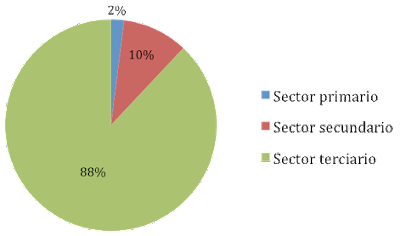
\includegraphics[width=0.5\textwidth]{Memoria_TFG_LaTeX/images/sectoresEconomicosCanarias.png}
    \caption{Distribución de la masa de trabajadores entre los diferentes sectores laborales en Canarias en el año 2020\cite{sectoresEconomicosCanarias}.}
    \label{fig:sectoresCanarias}
\end{figure}

Y en el siguiente diagrama, se observa el aporte del turismo al PIB\footnote{\textbf{PIB}:El producto interior bruto, o por sus siglas PIB, mide la producción total de bienes y servicios de un país. El PIB, por lo tanto, mide el tamaño de la economía de un país, es decir, toda su riqueza económica. Cuánto mayor es el PIB de un país, mayor es su capacidad económica y, por tanto, mayor es su capacidad para generar empleo e inversión.} canario.
\begin{figure}[H]
    \centering
    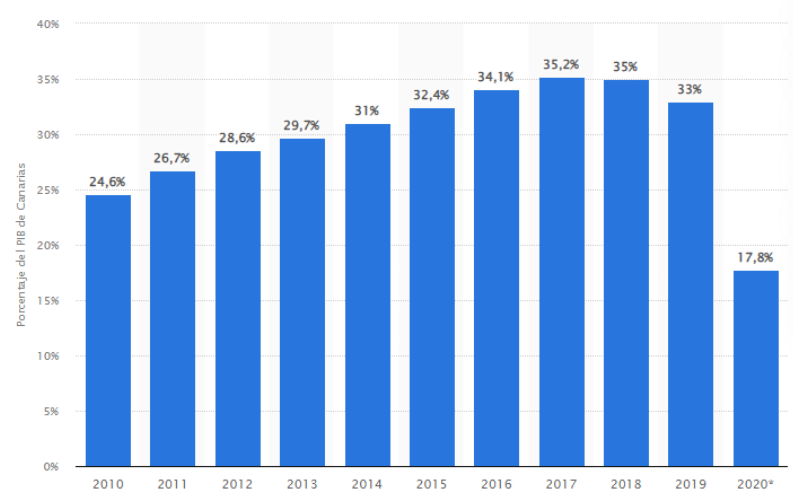
\includegraphics[width=0.5\textwidth]{Memoria_TFG_LaTeX/images/pibcanarias2010-2020.PNG}
    \caption{Aporte del turismo al PIB de canarias. \cite{PIBTurismoCanarias2010-2020}}
    \label{fig:PIB2010-2020}
\end{figure}

Durante los años de pandemia, ha habido un acentuado descenso en la cantidad de turistas que recibe el archipiélago canario. Se estima en un 88.33\% aproximadamente entre 2019 y 2020. 


Afortunadamente, actualmente nos encontramos en un periodo de recuperación económica. 
\begin{figure}[H]
    \centering
    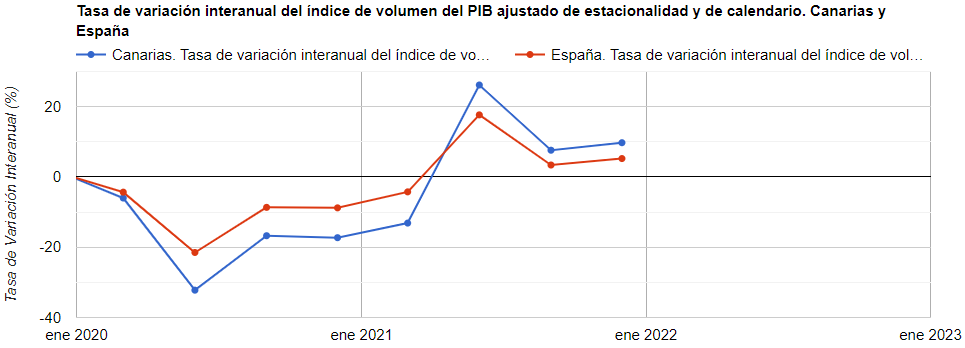
\includegraphics[width=1\textwidth]{Memoria_TFG_LaTeX/images/variacionPIB2020-2022.PNG}
    \caption{Variación del PIB canario entre los años 2020 y 2022. \cite{PIBInteranualCanarias2020-2022}}
    \label{fig:PIB2020-2022}
\end{figure}

Este proyecto pretende dar una motivación más tanto a turistas como a residentes para visitar los diferentes puntos de la Isla y así generar un mayor movimiento turístico en la zona.

%\href{http://www.gobiernodecanarias.org/istac/jaxi-istac/tabla.do?uripub=urn:uuid:ccdf465c-2230-421d-99f6-d6a1669d6032&uripx=urn:uuid:a4f8d3ed-fffc-4f58-b0bf-6ea6d2ab3d54}{info}

%\href{https://docs.google.com/spreadsheets/d/1GL6-trFgfcL-_D5phbUSWi1dCoglB_obWns4Yj6WN9Q/edit#gid=1515882426}{GoogleSheet}

\section{Justificación}

Esta aplicación puede motivar el turismo por la Isla de dos maneras:
\begin{itemize}
\item La primera es promocionando los sitios turísticos que se encuentran cerca del usuario, funcionando como una guía turística convencional, pero con las ventajas que la plataforma móvil ofrece, como pueden ser, la disponibilidad, la actualización constante de contenido, la portabilidad, etcétera.

\item La segunda es el entretenimiento que ofrece con la parte ludificada del proyecto. El mundo de los videojuegos está repleto de premios y logros que van recompensando al jugador por su curiosidad, interés y en definitiva, por seguir jugando \cite{porquenosgustanvideojuegos}. La aplicación presentada podría hacer que aquellos usuarios que sean coleccionistas que buscan completar todos esos premios intentasen completar el mapa de Tenerife, volviendo a generar movimiento por la Isla.

\end{itemize}

Otro factor importante que puede justificar el proyecto es promover el consumo de productos o servicios de kilómetro cero\footnote{\textbf{Producto de kilómetro cero}: Los alimentos, productos o servicios de kilómetro cero son aquellos elaborados a menos de 100 km del punto de venta.} como con las numerosas ventajas que ofrece este tipo de consumo. \cite{kilometro0} Como se comentará más adelante, sería posible incluir publicidad de establecimientos locales cercanos, como pueden ser restaurantes típicos como los denominados guachinches\footnote{\textbf{Guachinche}: es un establecimiento propio de la zona norte de la isla de Tenerife, en el que se ofrece comida casera tradicional, como acompañamiento al vino de cosecha propia o de la zona a precio reducido por ser comprado directamente al productor es este.} o tiendas de artesanía típica canaria, etc. De esta forma, se favorecería un turismo orientado al consumo local, que ayudaría a las pequeñas empresas locales y al disfrute de toda la naturaleza de la Isla. Gracias a tener acceso al GPS\footnote{\textbf{GPS}: Sistema de Posicionamiento Global (Global Positioning System) es un sistema que permite posicionar cualquier objeto sobre la tierra con una precisión de metros o incluso de centímetros.} del dispositivo del usuario este tipo de publicidad sería mucho más efectiva y mejor dirigida.

En los últimos años, este tipo de turismo parece haber aumentado en proporción al turismo más típico de "todo incluido"\cite{turismotodoincluido}. También durante los últimos años, el Gobierno de Canarias ha lanzado varias campañas para promover el cambio de modelo de turismo a uno en el que se consuman más productos locales \cite{campañaelaboradoencanarias}.

\section{Tendencia de mercado}
Como se ha comentado anteriormente, en la actualidad, nos encontramos en un periodo de recuperación turística de suma importancia. Ya que, durante los años de restricciones por la pandemia de Covid 19, el flujo de turistas se redujo prácticamente a cero. En el siguiente gráfico podemos observar ese descenso brusco del número de turistas durante los años 2020 y la recuperación de ese flujo de turistas durante el año 2021 en adelante.

\begin{figure}[H]
    \centering
    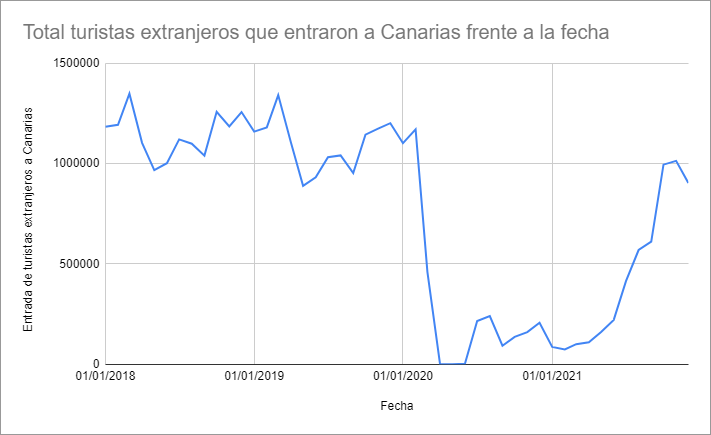
\includegraphics[width=1\textwidth]{Memoria_TFG_LaTeX/images/turistas2018-2022.png}
    \caption{Gráfico que muestra la entrada de turistas extranjeros a Canarias por año.}
    \label{fig:turistas}
\end{figure}

Se puede apreciar que se está comenzando a recuperar el nivel prepandémico.
Con lo cual, el año actual es el momento óptimo para lanzar una aplicación destinada a fortalecer el turismo, pues éste está en pleno auge a niveles prepandémicos.

\section{Estado actual y competencia}
Hoy en día, en la Google Play Store\footnote{\textbf{Google Play Store}:  Anteriormente llamado Android Market, es una plataforma de distribución digital de aplicaciones móviles para los dispositivos con sistema operativo Android, así como una tienda en línea desarrollada y operada por Google. Esta plataforma permite a los usuarios navegar y descargar aplicaciones (desarrolladas mediante Android SDK), juegos, música, libros, revistas y películas.} podemos encontrar varias guías turísticas. 
La mayoría de estas están en formato Ebook\footnote{\textbf{Ebook}: Se trata de una versión digitalizada de un libro, algunos Ebooks no tienen edición física.} lo que impide una mayor interacción por parte del usuario. Como los libros de guías turísticas tienen mayor tiempo en el mercado, estos poseen mayor prestigio o confianza a la vista de un usuario medio. Pero, por contraparte, este tipo de guías son más difíciles de actualizar con nuevos puntos de interés.
Ya existen algunas aplicaciones que hacen de guía turística disponibles en la plataforma, pero ninguna de ellas posee ese factor de gamificación o de recompensa al usuario por visitar esos lugares, más allá del disfrute del propio lugar. A continuación, se muestra una tabla que analiza las diferencias, ventajas y desventajas de las otras guías ya disponibles en comparación con mi propuesta.

\begin{ThreePartTable}
\label{table:competencia}
\captionof{table}{Comparativa del prototipo de DiscoverTenerife con la competencia}

\begin{tabularx}{0.9\textwidth} { 
  | >{\centering\arraybackslash}X 
  | >{\centering\arraybackslash}X
  | >{\centering\arraybackslash}X
  | >{\centering\arraybackslash}X
  | >{\centering\arraybackslash}X | }
 \hline
 Nombre & Ventajas & Desventajas & Similitudes & Diferencias\\
 \hline\hline
 Ebooks & Más experiencia y más renombre & De pago, no interactiva, solo lectura & Señala lugares de interés & No gamificada y no interactiva\\
\hline
Tenerife Guia Turística & Muy buenas valoraciones en Google Play Store, opciones para reservar en villas y hoteles, tiene navegador GPS interno para llegar a los lugares & No parece recordar si se ha visitado un lugar o no & Señala lugares de interés & Mi prototipo solamente incluirá parajes naturales o lugares públicos, no gamificado\\
\hline
Mapa de Tenerife offline + guía & Buenas valoraciones en Google Play Store funciona sin conexión a internet, tiene descripciones de cada ubicación & No parece recordar si se ha visitado un lugar o no & Señala lugares de interés & No gamificado, en la versión premium tiene sistema de navegación GPS, sistema de ubicaciones favoritas \\
\hline
Tenerife: Guía de viaje & Base de usuarios en Google Play Store & No parece recordar si se ha visitado un lugar o no & Señala lugares de interés & No gamificado, permite planificar visitas de varios días, incluye restaurantes, hoteles y tours \\
\hline
\end{tabularx}

\end{ThreePartTable}
\section{Objetivos}
Este estudio pretende responder a las siguientes preguntas: ¿Es rentable una aplicación móvil de guía turística ludificada con estas características? ¿Ayudará realmente a incrementar el turismo por la zona?

Para responder a esas preguntas se han planteado los siguientes objetivos:

\begin{itemize}

\item Analizar las herramientas software o tecnologías disponibles para llevar a cabo el desarrollo y seleccionar la más adecuada o conveniente.

\item Identificar la competencia y establecer una serie de características con las que destacar nuestro proyecto frente a las otras soluciones disponibles.

\item Desarrollo de arquitecturas:

    \begin{itemize}
    
    \item Desarrollar un Web Scraper que capture la información de los puntos de interés.
    
    \item Implementar aplicación en Android.
    
    
        \begin{itemize}
        
        \item Se muestran los puntos de interés más cercanos a la ubicación actual del usuario.
        
        \item Se detecta cuando un usuario ha visitado un punto de interés.
        
        \item Existen opciones para permitir que el usuario decida que puntos de interés ver.
        
        \item Existen opciones para permitir al usuario elegir como se ordenan los puntos de interés; de menor distancia a mayor o de más visitados por el conjunto de usuarios, a menos visitados.
        
        \end{itemize}
        
    
    \item Desarrollar Backend con el que conectará dicha aplicación.
    
        \begin{itemize}
            
        \item El usuario puede registrarse con email y contraseña o de forma anónima.
        
        \item La información relativa al usuario es almacenada en el servidor: qué lugares ha visitado y cuando.
        
        \item La información relativa a los puntos de interés es almacenada en el servidor: nombre, dirección, coordenadas geográficas, etc.
        
        \end{itemize}
    
    \item Desarrollar una página web sencilla que permita consultar la tabla de clasificación de los usuarios.
    
    \end{itemize}
\item Realizar las pertinentes pruebas al conjunto de la aplicación.

\item Desarrollar un plan de negocio para la comercialización del producto:

    \begin{itemize}
    
    \item Crear un Diagrama de Gantt\footnote{\textbf{Diagrama de Gantt}: es una herramienta gráfica cuyo objetivo es exponer el tiempo de dedicación previsto para diferentes tareas o actividades a lo largo de un tiempo total determinado. No muestra las relaciones entre las diferentes tareas.} con las tareas a realizar, su duración, sus recursos y su costo.
    
    \item Prever la inversión inicial del proyecto.
    
    \item Diseñar modelo de comercialización del producto.
    
    \item Calcular el ROI\footnote{\textbf{ROI}: El retorno sobre la inversión (ROI, por las siglas en inglés de return on investment) es una métrica financiera que compara el beneficio o la utilidad obtenida en relación con la inversión realizada, es decir, calcula a partir de qué punto un proyecto comienza a ser rentable recuperando el dinero invertido, tanto al comienzo como durante el proceso.}.
    
    \end{itemize}
    
\end{itemize}



